\documentclass[fontsize=10pt]{article}
\usepackage[margin=0.70in]{geometry}
\usepackage{lipsum,mwe,abstract}
\usepackage[T1]{fontenc} 
\usepackage[english]{babel} 
\usepackage{multicol} 
\usepackage{setspace}




\usepackage{fancyhdr} % Custom headers and footers
%\pagestyle{fancyplain} % Makes all pages in the document conform to the custom headers and footers
%\fancyhead{} 
%\fancyfoot[C]{\thepage} % Page numbering for right footer
\usepackage{lipsum}
\setlength\parindent{0pt} 
\usepackage{authblk} % For affiliation formatting
\usepackage{amsmath,amsfonts,amsthm} % Math packages
\usepackage{wrapfig}
\usepackage{graphicx}
\usepackage{float}
\usepackage{subcaption}
\usepackage{comment}
\usepackage{enumitem}
\usepackage{cuted}
\usepackage{sectsty} % Allows customizing section commands
\allsectionsfont{\normalfont \normalsize \scshape} % Section names in small caps and normal fonts

\renewenvironment{abstract} % Change how the abstract look to remove margins
 {\small
  \begin{center}
  \bfseries \abstractname\vspace{-.5em}\vspace{0pt}
  \end{center}
  \list{}{%
    \setlength{\leftmargin}{0mm}
    \setlength{\rightmargin}{\leftmargin}%
  }
  \item\relax}
 {\endlist}
 
\makeatletter
\renewcommand{\maketitle}{\bgroup\setlength{\parindent}{0pt} % Change how the title looks like
\begin{flushleft}
  \textbf{\@title}
  \@author \\ 
  \@date
\end{flushleft}\egroup
}
\makeatother

%% ------------------------------------------------------------------- 
\title{\centering
\Large Modern Interferometry Executive Summary \\
[10pt] 
}


\author{\centering  Gordie Novak, Roxanne Ring, Natalie Gonzalez} 

\makeatletter
\renewcommand{\maketitle}{\bgroup
\setlength{\parindent}{0pt} % Change how the title looks like
\begin{flushleft}
  \textbf{\@title}
  \vspace{0.5em}
  \@author \\
  \vspace{1em}
  St. Olaf College
  \vspace{1em}
  
\end{flushleft}\egroup
}
\makeatother


\begin{document}

\maketitle

% --------------- ABSTRACT
\begin{abstract}

We aimed to analyze different topologies of the Michelson and Sagnac modern interferometries. Aligning lasers and using an oscilloscope to detect laser throughput results in electromagnetic interference patterns for both setups. Manipulating breadboard architecture, displacement mounts, time delays, and optical coherence serves as the basis for measurements with interferometers. The Michelson interferometer leverages mirror offsets to produce desirable interferences patterns, which we subsequently captured on the oscilloscope, the data then manipulated to calcualte wavelength of a HeNe laser, which we found to be [INSERT WAVELENGTH HERE]. The Sagnac interferometer, in which two beams travel identical paths in opposite directions, allows measurement of sensitivity to phase difference alone. Thus, we show that this interfermoter achieves a phase difference of $\Delta\phi$, by splittin g it into a bipolar electrical signal defined by $S \propto \cos(\Delta\phi)$. Thus, with a change in phase $\delta(\Delta\phi)$, we find an output signal $S$ will change by an amount $\delta S = \pm S_\text{max}\delta(\Delta\phi)$. Both of the interferometers demanded multilayer dielectric coatings, kinematic mountings, and flexure based mountings for success.
     
    
\end{abstract}

\rule{\linewidth}{0.5pt}

\begin{multicols}{2}

% --------------- MAIN CONTENT

\section{Introduction}
    Interferometry means “to measure using interference”. It’s a broad class of optical techniques that use the superposition of light waves to make extremely precise measurements. These techniques work by dividing a beam into a light of two separated beams that will travel along different paths and are later recombined. When the beams recombine, the beams might interfere constructively or destructively depending on their phase. A phase difference of 180 will result in destructive interference, while smaller phase shifts will result in measurable changes in the intensity of the laser. Interferometry is also directly related to optical path length, making it very sensitive and requiring extreme precision. A time delay or a path difference of half of wavelength is enough to switch between constructive and destructive interference. The small-scale precision of interferometers (in the range of nanometers) provide great experimental utility for measurement of microscopic phenomena. 
    
To properly create effective inferometers, we focused on optical alignment, component mounting, and the use of polarization to control the beam. Thus, we performed an exercise in "Modern" Interferometry due to our usage of lasers, electronic detection, and modern optical components.

We primarily investaged two interferometer variations: The Michelson and Sagnac. Although both provide opportunity to utilize the interference behavior of electromagnetic waves to measure small distances, their primary methodologies for achiving this goal vary considerably.

 	The \textbf{Michelson interferometer} splits a single laser beam into two perpendicular paths using a beamsplitter, with each beam reflected back by a mirror before recombining at the beamsplitter. The resulting interference pattern depends on the relative optical path lengths of the two arms, making the Michelson interferometer extremely sensitive to small changes in distance, refractive index, or mirror position. This sensitivity has made it an important tool for precision length measurements and tests of the nature of light and space-time.
    
	 The \textbf{Sagnac interferometer} divides a beam into two components that travel in opposite directions around a closed loop before recombining. With a well-constructed Sagnac interferometer, beam output depends \textit{exclusively on phase difference} and not on confounding factors such as mirror vibrations or air effects. Thus, if the interferometer is rotating, the two counter propagating beams experience different 'effective' path lengths, even though distance has not changed. This then produces a measurable phase shift in the interference signal.
     
We begin the analysis of data with the results from the Michelson Interferometer, followed by the Sagnac Interferometer. 




\section{Initial Discussion of Data}

The Michelson Interferometer's setup relies on the principle of two separate lasers following different paths to achieve a path length difference, resulting in a phase different upon incidence. Depicted in Figure 1 is the working setup utilized for the Interferometer.\\
However, a primary drawback of the Michelson interferometer is that it extremely susepctible to small variations in the environment. Various factors greatly decrease the effectiveness of this interferometer:\vspace{-0.2cm}
\begin{enumerate}[itemsep=0pt]
	\item \textbf{Vibration.} Any vibration in the envrionment greatly reduces interferometer stability.\vspace{-0.1cm}
	\item \textbf{Air-Density.} Working in an environment with inconsistent air density between either two arms of the interferometer (refer to Fig. 1) results in greater inconsistency. \vspace{-0.1cm}
	\item \textbf{Temperature.} Due to the nature of the Alumnimum Breadboard, warmth from hands is enough to warp the metal and change its dimension due to thermal contraction. 
\end{enumerate}
\begin{figure}[H]
    \centering
    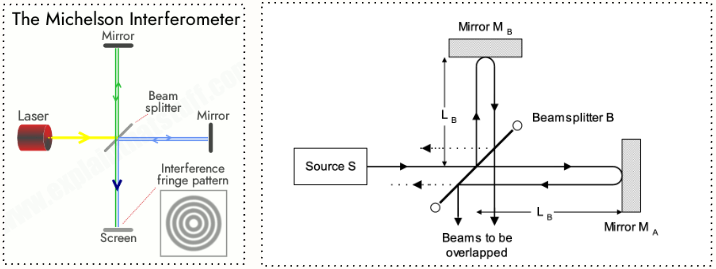
\includegraphics[scale=0.42]{images/Michelson-Inter.png}
    \caption{This image depicts the setup of the Michelson interferometer. The lasers constructively and destructively interfere at the same time with itself as it reflects off of the mirror, traveling in the opposite direction along the same path it was incoming, with marginal space between the incoming and outgoing beams to get interference along the fringes.}
\end{figure}
Thus, because of many of these various factors, the measurements provided by this interferometer were inconsistent and largely unreliable. As seen in Figure 2, this effect is dramatic. 
\begin{figure}[H]
    \centering
    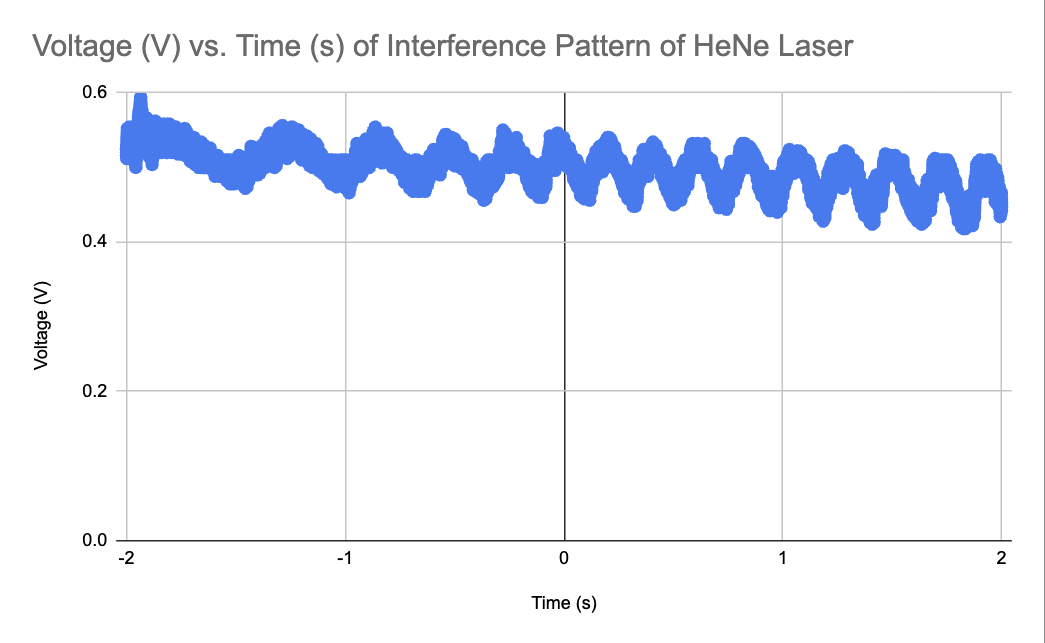
\includegraphics[scale=.21]{images/Michelson-Graph.png}
    \caption{Display of the inconsistency of the Michelson Interferometer signal. There are a total of 15 interference variations, average 7.5 per second.}
    \label{fig:inconsistency}
\end{figure}\
Manually adjusting the x
\begin{figure}[H]
    \centering
    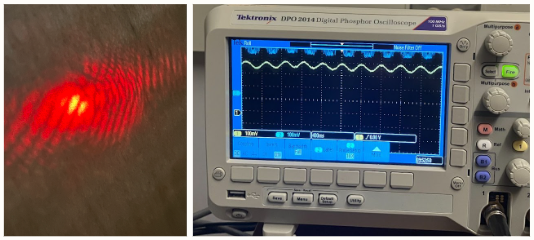
\includegraphics[scale=.52]{images/Interference-Pat.png}
    \caption{Depicts the visual and qualitative results of the experiment. Visually, we achieved a broad interference pattern along the fringes of the laser, and quantitatively the oscilloscopes readings reflected these results back displaying a consistent and refined oscillatory pattern. The distance between peaks was measured to be 654.22 nm using the translation stage and motor, which was in our desired range of 645-650 nm from other experimental values.}
    \label{fig:placeholder}
\end{figure}\

\begin{figure} [H]
    \centering
    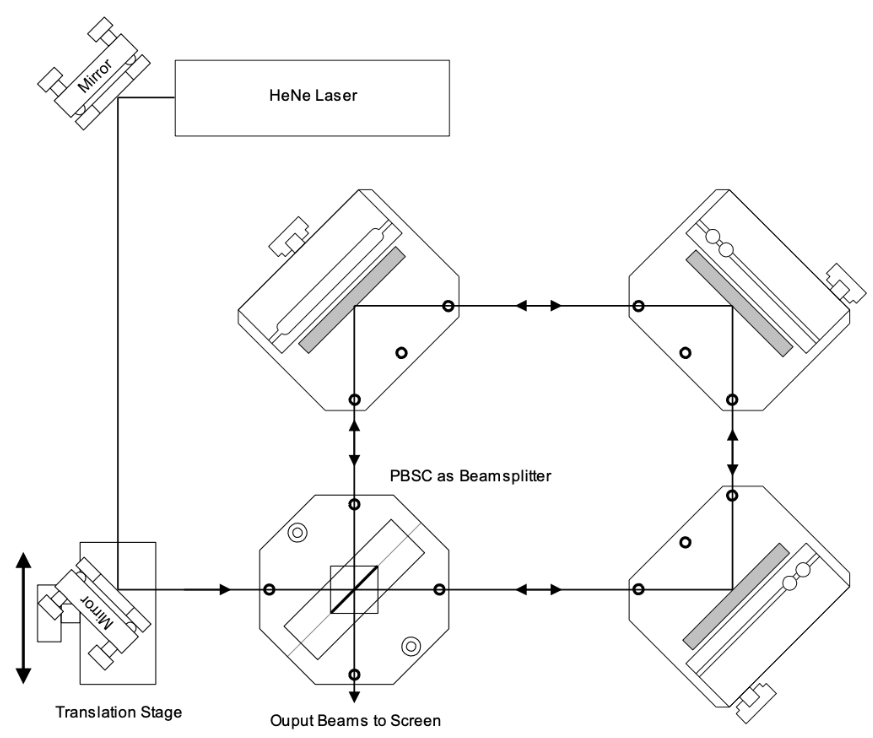
\includegraphics[scale=.30]{images/Experimental-setup.png}
    \caption{The topology of the Sagnac interferometer. This setup allowed for little more than microns of error, as the desired setup had the beams inward and outgoing beams along the exact same path and any slight deviation from this would result in failed data.}
    \label{fig:placeholder}
\end{figure}

\begin{figure}[H]
    \centering
    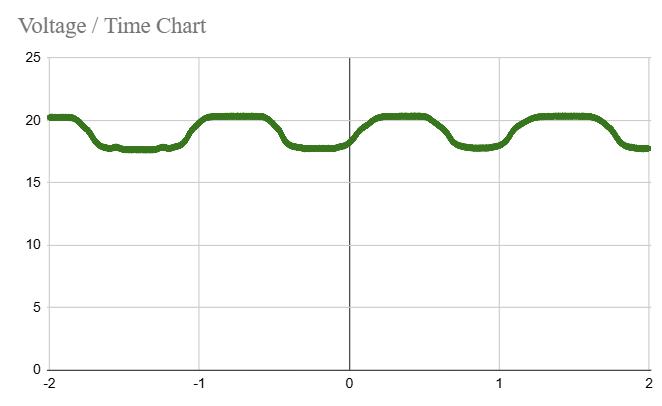
\includegraphics[width=0.5\linewidth]{images/Voltage vs. time.png}
    \caption{This was the data collected from translating mirror M2 along the translation stage of the Saganc interferometer setup. This back and forth translation of the mirror mimicked a rotation of the entire setup to exploit this difference in speeds of the light traveling in one direction of the path compared to the other, resulting in these long undulations in voltage over time.}
    \label{fig:placeholder}
\end{figure}

\section{Summary of Data}
\
For the Michelson interferometer, to calculate the wavelength of the HeNe laser, we needed to mount a horizontal mirror on a translation stage. We used a micrometer to measure the distance the translation stage moved and g=how many seconds 


\section{Discussion }












\section{Author Contributions}









\vspace{1pt}


\end{multicols}
\end{document}
 


